\documentclass[12pt]{article}
\usepackage[margin=1in]{geometry}
\usepackage{amsmath}
\usepackage{graphicx}
\usepackage{parskip}

\title{\textbf{LUP Decomposition}}
\author{}
\date{}

\begin{document}

\maketitle

In practice, the use of typical Gaussian elimination is the backbone for many physical and scientific
applications that involve the solving of linear systems with respect to the form $Ax = b$. This
algorithm in theory would solve in $\mathcal{O}(N^3)$, where looping through the rows and columns,
plus the back-substitution would create a triple nested for-loop. However, in the case of using a
symmetric positive definite (SPD) matrix, we can further break and decompose this process down into
segmented parts for solving using the LUP algorithm, which would result in a speed optimization.

Analyzing the graphs and results from timing, the LUP algorithm follows a similar but differing
growth pattern to $\mathcal{O}(N^3)$. At sample size $N = 10$ the runtimes are practically
identical to the reference curve; however, the interesting behavior lies at $N = 100$. In this test
case, the slope of work done to solve the system is more akin to the complexity of
$\mathcal{O}(N^2)$. This is likely due to the fact that since $N$ is moderately sized, the
algorithm's runtime is dominated by the forward and backward substitution steps, which each solve in
$\mathcal{O}(N^2)$, while the decomposition itself contributes a cost closer to
$\mathcal{O}(\frac{1}{3}N^3)$ --- small enough at this scale to be masked. This explanation is
further supported by the behavior at $N = 1000$, where the empirical slope rises to approximately
$\mathcal{O}(N^{3.5})$. This super-cubic growth is attributed more to memory access patterns and
cache latency than to the algorithm itself, as the working set exceeds cache capacity and main-memory
bandwidth becomes a bottleneck. Regardless, this case study demonstrates that with proper scaling,
LUP decomposition can be reliably deployed for the efficient solving of linear systems of the form
$Ax = b$.

\begin{figure}[h]
    \centering
    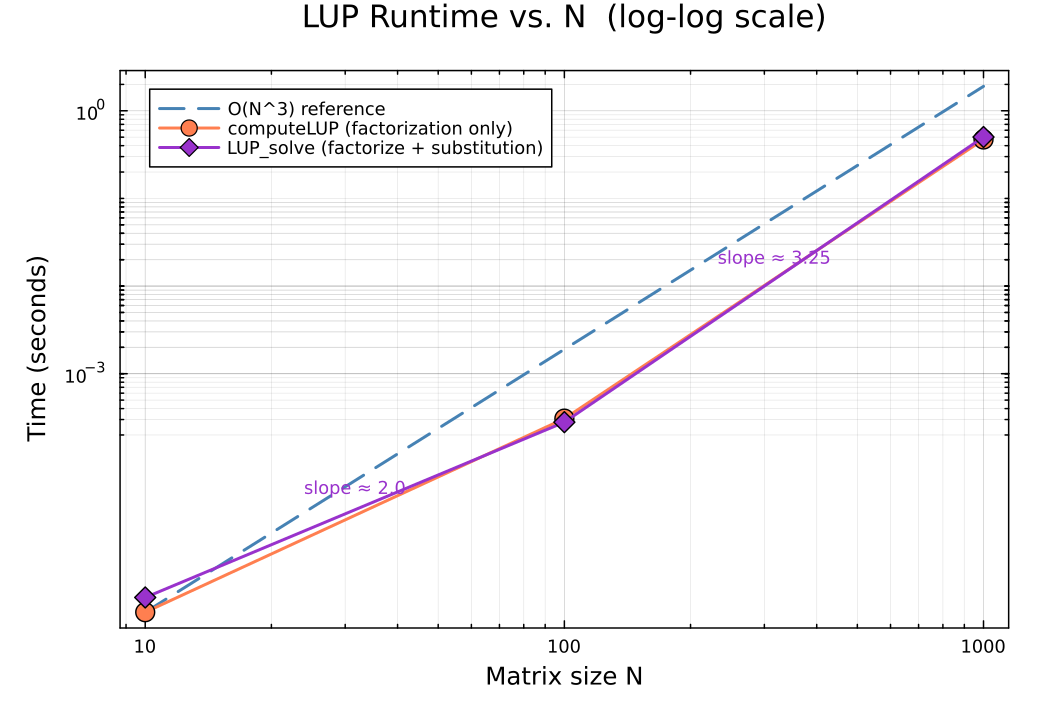
\includegraphics[width=0.85\textwidth]{lup_timing.png}
    \caption{Runtime of \texttt{computeLUP} and \texttt{LUP\_solve} as a function of matrix size
    $N$ on a log-log scale. The dashed line shows the $\mathcal{O}(N^3)$ reference anchored to the
    $N = 10$ measurement. Empirical slopes are annotated on each segment of the
    \texttt{LUP\_solve} curve.}
    \label{fig:lup_timing}
\end{figure}

\end{document}
